\documentclass[12pt]{article}


\usepackage{amssymb}
\usepackage{amsmath}
\usepackage{fullpage}
\usepackage{epsfig}
\usepackage{epstopdf, hyperref, xcolor}
\everymath{\displaystyle}

\newif\ifans

\anstrue

\begin{document}

\begin{center}
\underline{\LARGE{The Definite Integral}}
\end{center}

\noindent SUGGESTED REFERENCE MATERIAL:

\bigskip

\noindent As you work through the problems listed below, you should reference Chapter 5.5 of the recommended textbook (or the equivalent chapter in your alternative textbook/online resource) and your lecture notes.

\bigskip

\noindent EXPECTED SKILLS:

\begin{itemize}

\item Be able to evaluate the definite integral of a function over a given interval using geometry.

\item Be familiar with the interpretation of the definite integral of a function over an interval as the net signed area between the graph of the function and the $x$-axis.

\item Know how to use linearity properties of the definite integral to evaluate scalar multiples, sums, and differences of integrable functions.  

\end{itemize}

\noindent PRACTICE PROBLEMS:

\medskip

\noindent {\bf For problems 1 \& 2, use the given values of $a$ and $b$ to express the given limit as a definite integral. Do not evaluate the limits or integrals.}

\begin{enumerate}

\item $\lim_{\max \Delta x_k \rightarrow 0} \sum_{k=1}^n \frac{1}{1+(x_k^*)^2} \Delta x_k$, $a=-1$, $b=1$.

\ifans{\fbox{$\int_{-1}^1{\frac{1}{1+x^2}} \,dx$}} \fi

\item $\lim_{\max \Delta x_k \rightarrow 0} \sum_{k=1}^n \cos{(x_k^*)} \Delta x_k$, $a=0$, $b=\pi$.

\ifans{\fbox{$\int_0^{\pi}\cos{x} \,dx$}} \fi

\end{enumerate}

\noindent {\bf For problems 3-9, sketch the region whose net signed area is represented by the given definite integral.  Evaluate the given integral using an appropriate formula from geometry.}

\begin{enumerate}
\setcounter{enumi}{2}

\item $\int_0^7{(x+1)}\,dx$

\ifans{\fbox{$\frac{63}{2}$}} \fi

\item $\int_{-7}^7{x}\,dx$

\ifans{\fbox{$0$}} \fi

\item $\int_{-1}^4{6}\,dx$

\ifans{\fbox{$30$}} \fi

\item $\int_{-4}^{2}{|x-1|} \,dx$

\ifans{\fbox{$13$}} \fi

\item $\int_{-2}^2{\sqrt{4-x^2}} \,dx$

\ifans{\fbox{$2\pi$}} \fi

\item $\int_{-2}^0{\left(3x+5\sqrt{4-x^2}\right)} \,dx$

\ifans{\fbox{$-6+5\pi$; Detailed Solution: \textcolor{blue}{\href{http://www.math.drexel.edu/classes/Calculus/resources/Math122HW/Solutions/122_02_Definite_08.pdf}{Here}}}} \fi

\item $\int_4^8{\sqrt{8x-x^2}} \,dx$

\ifans{\fbox{$4\pi$}} \fi

\item Let $f(x)=\left\{\begin{array}{lll}
3x & \text{ if} & x \leq 2 \\
6 & \text{ if} & x>2
\end{array}\right.$.  Compute $\int_{-1}^5{f(x)} \,dx$.

\ifans{\fbox{$\frac{45}{2}$; Detailed Solution: \textcolor{blue}{\href{http://www.math.drexel.edu/classes/Calculus/resources/Math122HW/Solutions/122_02_Definite_10.pdf}{Here}}}} \fi

\item For each of the following, use the areas shown to evaluate the given definite integral.

\begin{center}

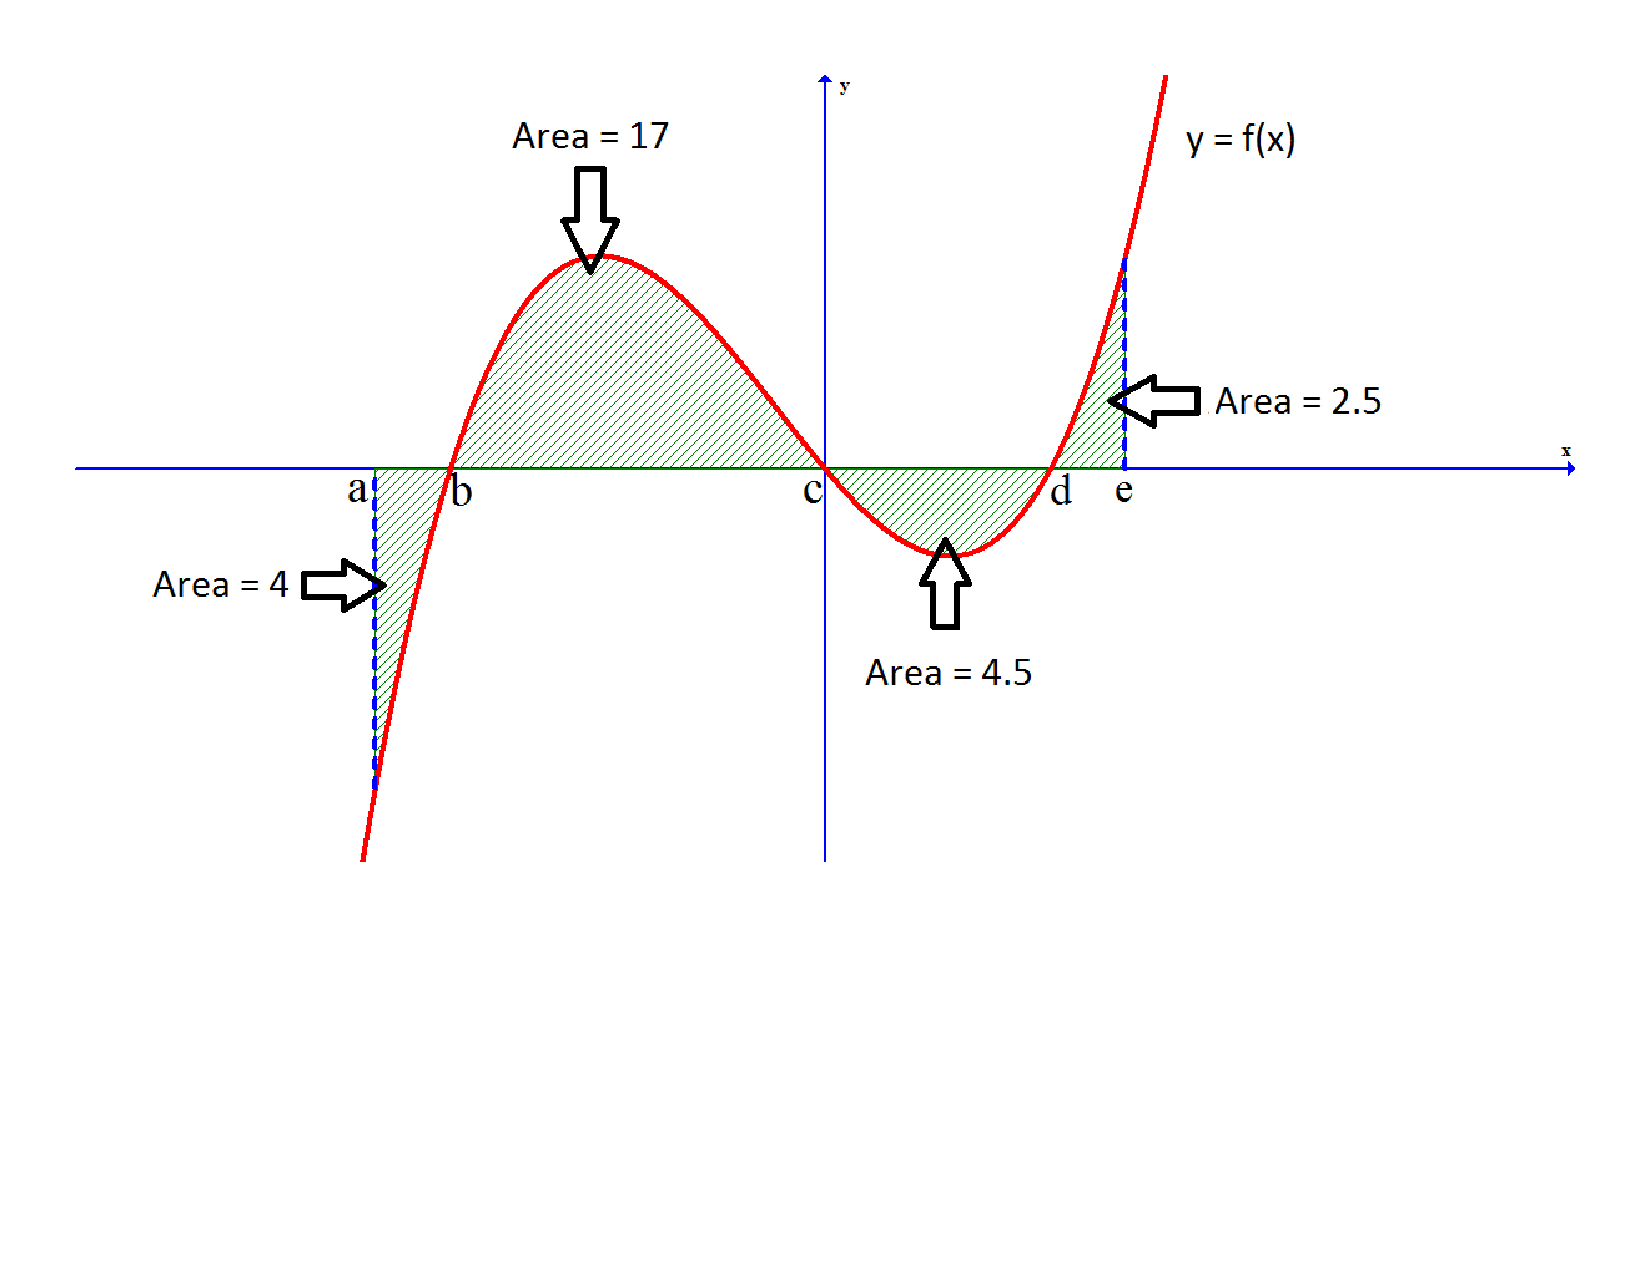
\includegraphics[scale=0.4]{area_graph.pdf}

\end{center}

\begin{enumerate}

\item $\int_b^c{f(x)} \,dx$

\ifans{\fbox{$17$}} \fi

\item $\int_c^d{f(x)} \,dx$

\ifans{\fbox{$-4.5$}} \fi

\item $\int_a^e{f(x)} \,dx$

\ifans{\fbox{$11$}} \fi

\item $\int_b^a{f(x)} \,dx$

\ifans{\fbox{$4$}} \fi

\end{enumerate}

\item Again consider the graph of $y=f(x)$ shown in problem 11.  Compute $\int_a^e{|f(x)|} \,dx$ and $\left|\int_a^e{f(x)} \,dx \right|$.  Which is larger?

\ifans{\fbox{$\int_a^e|f(x)| \,dx=28$; $\left|\int_a^e{f(x)} \,dx\right|=11$; $\int_a^e{|f(x)|} \,dx$ is larger.}} \fi

\item Suppose that $\int_{-1}^3{f(x)} \,dx=6$ and $\int_{-1}^{3}{g(x)} \,dx=-8$.  Compute $\int_{-1}^3{(f(x)+4g(x))} \,dx$.

\ifans{\fbox{$-26$}} \fi

\item Suppose that $\int_0^8{f(x)} \,dx=3$ and $\int_4^{8}{f(x)} \,dx=10$.  Compute $\int_0^4{f(x)} \,dx$.

\ifans{\fbox{$-7$}} \fi

\item Suppose that $\int_{-2}^9{f(x)} \,dx=4$ and $\int_{-2}^{6}{f(x)} \,dx=11$.  Compute $\int_{9}^6{f(x)} \,dx$.

\ifans{\fbox{$7$; Video Solution: \textcolor{blue}{\href{https://www.youtube.com/watch?v=IBZspjDFQmY}{https://www.youtube.com/watch?v=IBZspjDFQmY}}}} \fi

\item Express each of the following in terms of $\int_0^{\pi}\sin{x} \,dx$.  {\bf Do not evaluate any of the integrals.}  Hint: Draw a graph and consider the net signed area.

\begin{enumerate}

\item $\int_{\frac{\pi}{2}}^{\frac{3\pi}{2}}\cos{x} \,dx$.

\ifans{\fbox{$\int_{\frac{\pi}{2}}^{\frac{3\pi}{2}}\cos{x} \,dx=-\int_0^{\pi}\sin{x} \,dx$}} \fi

\item $\int_{\frac{3\pi}{2}}^{2\pi}\cos{x} \,dx$.

\ifans{\fbox{$\int_{\frac{3\pi}{2}}^{2\pi}\cos{x} \,dx=\frac{1}{2}\int_0^{\pi}\sin{x} \,dx$}} \fi

\item $\int_{\pi}^{\frac{3\pi}{2}}\sin{x} \,dx$.

\ifans{\fbox{$\int_{\pi}^{\frac{3\pi}{2}}\sin{x} \,dx=-\frac{1}{2}\int_0^{\pi}\sin{x} \,dx$}} \fi

\end{enumerate}

\item Suppose $F(x)=\int_0^x{f(t)} \,dt$, where $f(t)$ is shown below.

\hspace{2cm} 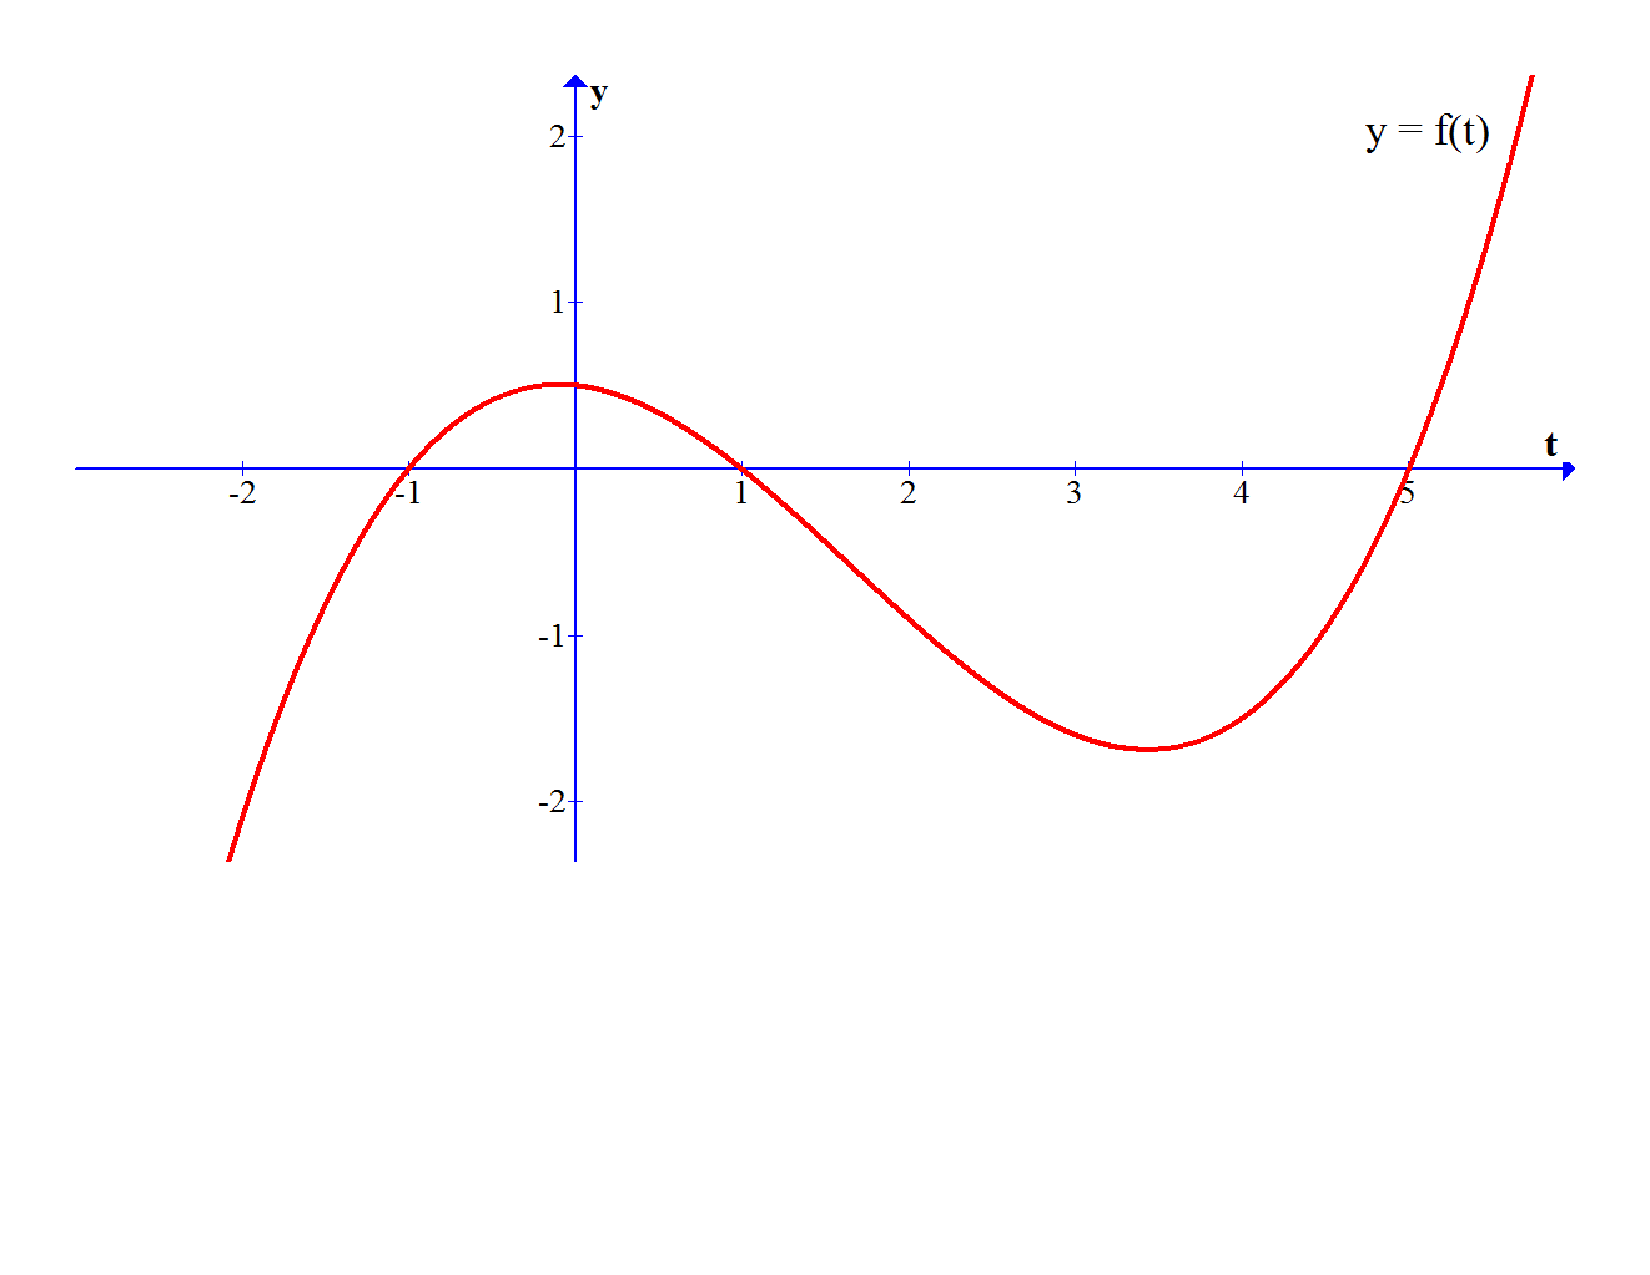
\includegraphics[scale=0.4]{graph2.pdf}

Arrange the following quantities in order from least to greatest. $F(0)$, $F(1)$, $F(5)$, $F(1)-F(5)$, $F(5)-F(1)$

\ifans{\fbox{$F(5)-F(1)<F(5)<F(0)<F(1)<F(1)-F(5)$}} \fi

\item The following Riemann Sum was derived by dividing an interval $[a,b]$ into $n$ subintervals of equal width and then choosing $x_k^*$ to be the right endpoint of each subinterval.

$$\lim_{n \rightarrow +\infty} \sum_{k=1}^n{\left(1+\frac{4}{n}k\right)\frac{4}{n}}$$

\begin{enumerate}

\item What is the interval, $[a,b]$?

\ifans{\fbox{If we consider $f(x)=x$, then the interval is $[1,5]$.}} \fi

\item Convert the Riemann Sum to an equivalent definite integral.

\ifans{\fbox{$\lim_{n \rightarrow +\infty} \sum_{k=1}^n{\left(1+\frac{4}{n}k\right)\frac{4}{n}}=\int_1^5{x} \,dx$}} \fi

\item Using the definite integral from part (b) and an appropriate formula from geometry, evaluate the limit.

\ifans{\fbox{12}} \fi

\end{enumerate}

\ifans{{\bf NOTE:} In number 18, there are many correct answers.  For example, we could have considered $f(x)=1+x$.  In that case, $[a,b]=[0,4]$ and $\lim_{n \rightarrow +\infty} \sum_{k=1}^n{\left(1+\frac{4}{n}k\right)\frac{4}{n}}=\int_0^4{(1+x)} \,dx$.  The value of this definite integral is also 12.} \fi

\end{enumerate}

\end{document}